  \clearpage
  %%%%%%%%%%%%%%%%%%%%%%%%%%%%%%%%%%%%%%%%%%%%%%%%%%%%%%%%%%%%%%%%%%%%%%%%%%%%%%%%%
  %%        %%%        %%%        %%%        %%%        %%%         %%%  %%%%  %%%
  %%  %%%%%%%%%  %%%%%%%%%  %%%%%%%%%%%%  %%%%%%%%%  %%%%%%  %%%%%  %%%    %%  %%%
  %%        %%%        %%%  %%%%%%%%%%%%  %%%%%%%%%  %%%%%%  %%%%%  %%%  %  %  %%%
  %%%%%%%%  %%%  %%%%%%%%%  %%%%%%%%%%%%  %%%%%%%%%  %%%%%%  %%%%%  %%%  %%    %%%
  %%        %%%        %%%        %%%%%%  %%%%%%        %%%         %%%  %%%   %%%
  %%%%%%%%%%%%%%%%%%%%%%%%%%%%%%%%%%%%%%%%%%%%%%%%%%%%%%%%%%%%%%%%%%%%%%%%%%%%%%%%%
 \section{任意の関数に従うヒストグラムを描く}
 自分で定義した関数に従って乱数を生成してヒストグラムを描こう。
 \begin{itembox}{\texttt{ranfun.cpp}}
\begin{verbatim}
	#include "TCanvas.h"
	#include "TF1.h"
	#include "TH1.h"
	#include "TMath.h"
	TH1D *ranfun(){
	double range_min = 0. ; // 0 [ns]
	double range_max = 8000.e-9 ;// 8000 [ns]
	double tau       = 2.2e-6 ; // it means lifetime
	double bgd = 0.5 ; // Background
	int nbin = 100 ; // histgram bin num
	int imax = 100000 ; // event

	TCanvas *c1 = new TCanvas("c1","c1",600,600) ;
	c1->SetGrid(1,1) ; // Canvas c1 にグリッドを描く
	c1->SetLogy(1) ;  // Canvas c1 の縦軸をlogで

	TF1 *f = new TF1("f","TMath::Exp(-x/[0])+[1]", range_min, range_max) ;
	f->SetParameter(0, tau) ;
	f->SetParameter(1, bgd) ;
	//  f->SetParameters(tau,bgd) ; // <--上の二行はこの一行と等価

	TH1D *h = new TH1D("h","Decay curve (Muon);TDC [s] ; Counts ", nbin, range_min, range_max) ;
	for(int i=0; i < imax; i++){
	h->Fill(f->GetRandom()) ;
	}
	h->Draw("HE") ;

	/********************************************************************************\
	* Decay Curve Fitting
	\********************************************************************************/
	/* If you want to use fit, then please uncomment
	gStyle->SetOptFit(1101) ;
	TF1 *muon = new TF1("muon","[0]*TMath::Exp(-x/[1])+[2]") ;
	muon->SetParameters(2e+3, 2e-6, 1e+2) ;
	muon->SetLineColor(kBlue) ;
	muon->SetLineWidth(4) ;
	h->Fit(muon) ;
	*/
	return h ;
	}
\end{verbatim}
 \end{itembox}

  \subsection{練習}
  \begin{enumerate}
   \item プログラムの各行の役割を理解せよ。
	 \begin{description}
	  \item[ヒント] \url{http://root.cern.ch/root/html/TF1.html#TF1:GetRandom}
	 \end{description}

   \item 図\ref{Fig:ranfunsol1canvas1}のようなおしゃれをしたヒストグラムを描け。
	 \begin{figure}[htbp]
	  \begin{center}
	   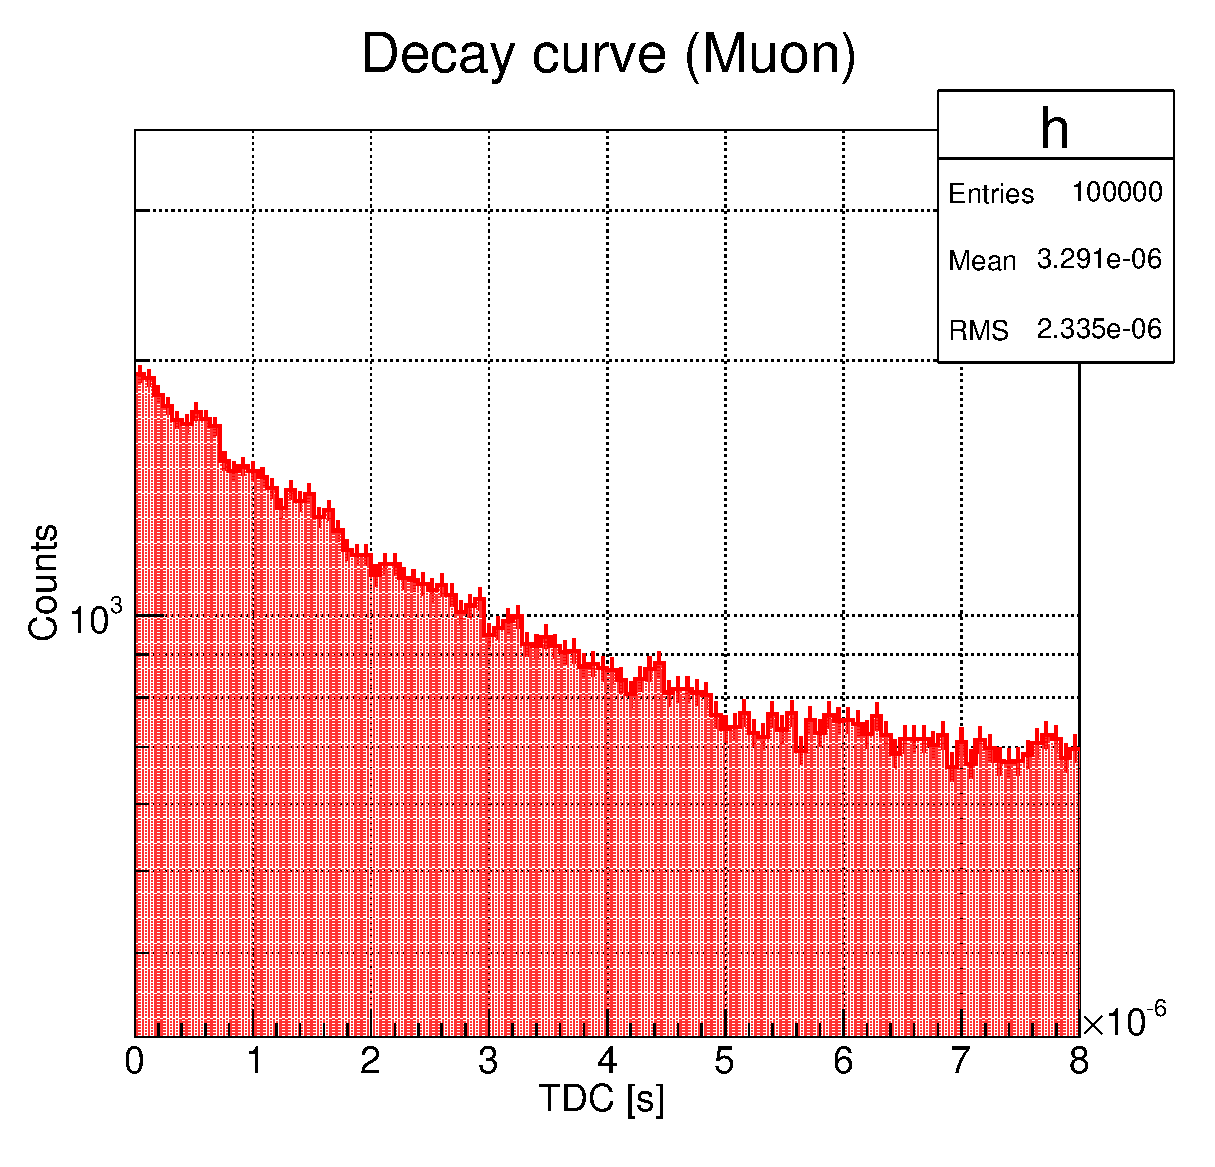
\includegraphics[width = 90mm]{./picture/ranfunsol1canvas1.eps}
	  \end{center}
	  \caption{各種の設定をいじったヒストグラム}
	  \label{Fig:ranfunsol1canvas1}
	 \end{figure}
	 \begin{description}
	  \item[ヒント] \url{http://root.cern.ch/root/html/TH1.html#TH1:GetXaxis}
	  \item[ヒント] \url{http://root.cern.ch/root/htmldoc/TAxis.html#TAxis:CenterTitle}
	  \item[ヒント] \url{http://root.cern.ch/root/html/TH1.html#TH1:SetTitleOffset}
	  \item[ヒント] \url{http://root.cern.ch/root/html/TAttFill.html#TAttFill:SetFillColor}
	  \item[ヒント] \url{http://root.cern.ch/root/html/TAttFill.html#TAttFill:SetFillStyle}
	 \end{description}

   \item \verb|ranfun.cpp|の下部\verb|Decay Curve Fitting|以下のコメントアウトされている箇所\verb|/* ... */|をアンコメントして実行してみよ。
	 \begin{description}
	  \item[ヒント] この状態で\verb|ranfun.cpp|をコンパイルオプション付きでロードしたらエラーメッセージが出るだろう。
		     何を\verb|include|すべきかはコンパイラが認識し兼ねている単語と'ライブラリ'などの言葉と一緒に検索せよ。
		     それが\ROOT に関連しているものであれば各\verb|class|を説明しているページの右上に何を\verb|include|すべきかが書いてある。\\
		     \url{http://root.cern.ch/root/html/TStyle.html}
	 \end{description}
	 \begin{figure}[htbp]
	  \begin{center}
	   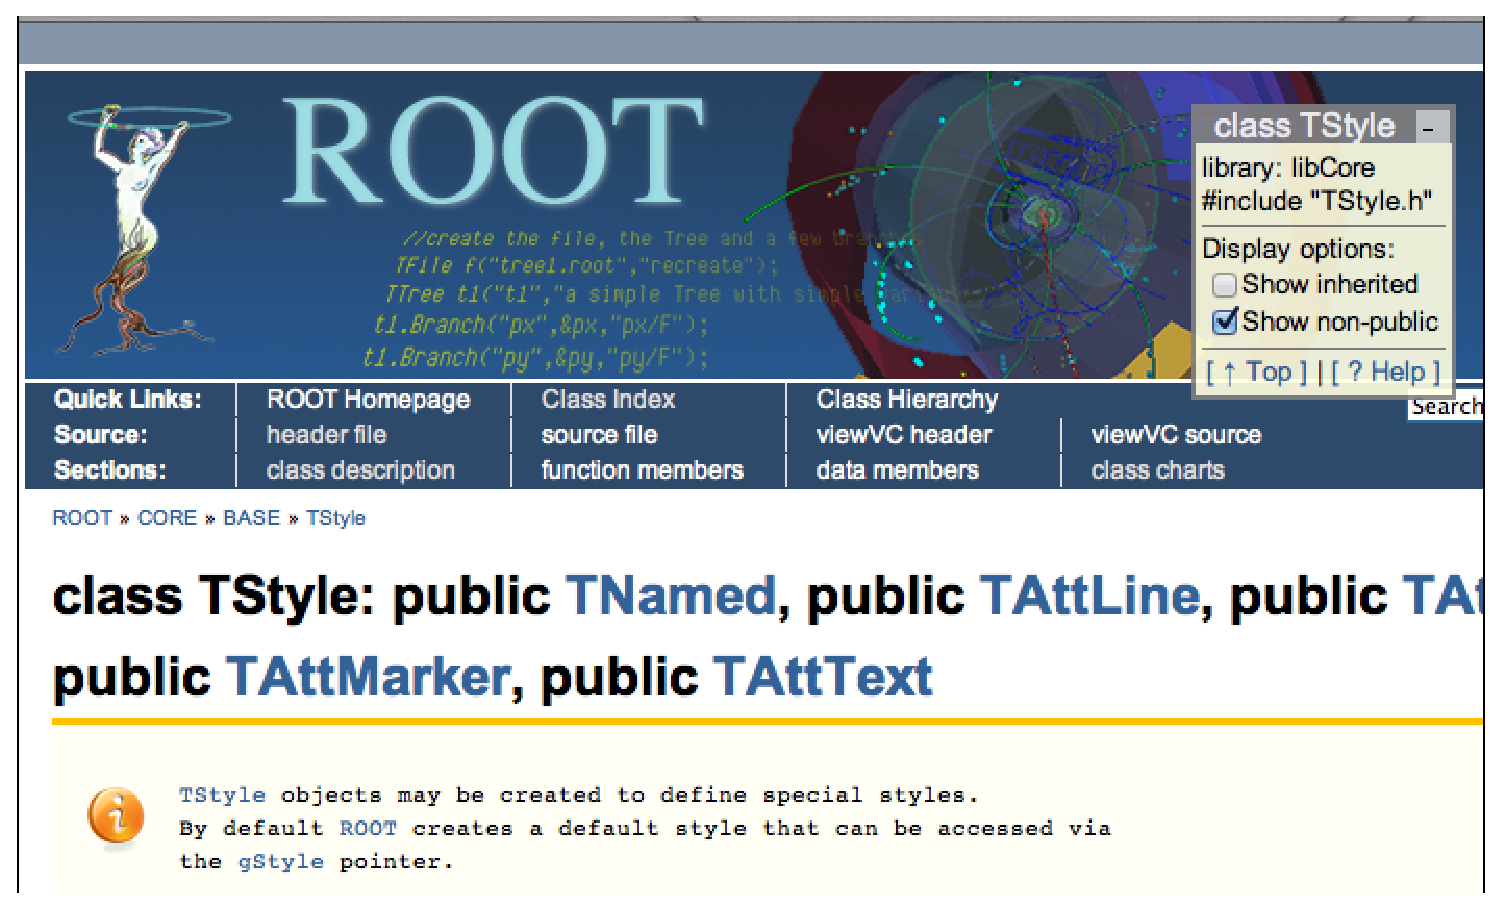
\includegraphics[width = 90mm]{./picture/classinclude.eps}
	  \end{center}
	  \label{Fig:classinclude}
	 \end{figure}
   \item フィッティングの情報が誤差付きで描かれるように変更せよ。
	 \begin{description}
	  \item[ヒント]  \url{http://root.cern.ch/root/html/TStyle.html#TStyle:SetOptFit}
	 \end{description}
  \end{enumerate}

  \subsection{解答例}

  \begin{enumerate}
   \item プログラムの各行の役割を理解せよ。

   \item 図\ref{Fig:ranfunsol1canvas1}のようなおしゃれをしたヒストグラムを描け。
	 \begin{itembox}{\texttt{ranfunsol1.cpp}}
\begin{verbatim}
	...
	TH1D  *ranfunsol1(){ 
	...
	h->GetXaxis()->CenterTitle() ;
	h->GetYaxis()->CenterTitle() ;
	h->GetYaxis()->SetTitleOffset(1.4) ;
	h->SetFillStyle(3002) ;
	h->SetFillColor(kRed-4) ;
	h->SetLineColor(kRed) ;
	h->SetLineWidth(2) ;
	...
	}
\end{verbatim}
	 \end{itembox}

   \item \verb|ranfun.cpp|の下部\verb|Decay Curve Fitting|以下のコメントアウトされている箇所\verb|/* ... */|をアンコメントして実行してみよ。

   \item フィッティングの情報が誤差付きで描かれるように変更せよ。
	 \begin{itembox}{\texttt{ranfunsol2.cpp}}
\begin{verbatim}
	...
	TH1D  *ranfunsol2(){ 
	...
	// If you want to use fit, then please uncomment
	gStyle->SetOptFit(1111) ;
	TF1 *muon = new TF1("muon","[0]*TMath::Exp(-x/[1])+[2]") ;
	muon->SetParameters(2e+3, 2e-6, 1e+2) ;
	muon->SetLineColor(kBlue) ;
	muon->SetLineWidth(4) ;
	h->Fit(muon) ;
	...
	}
\end{verbatim}
	 \end{itembox}
	 \begin{figure}[htbp]
	  \begin{center}
	   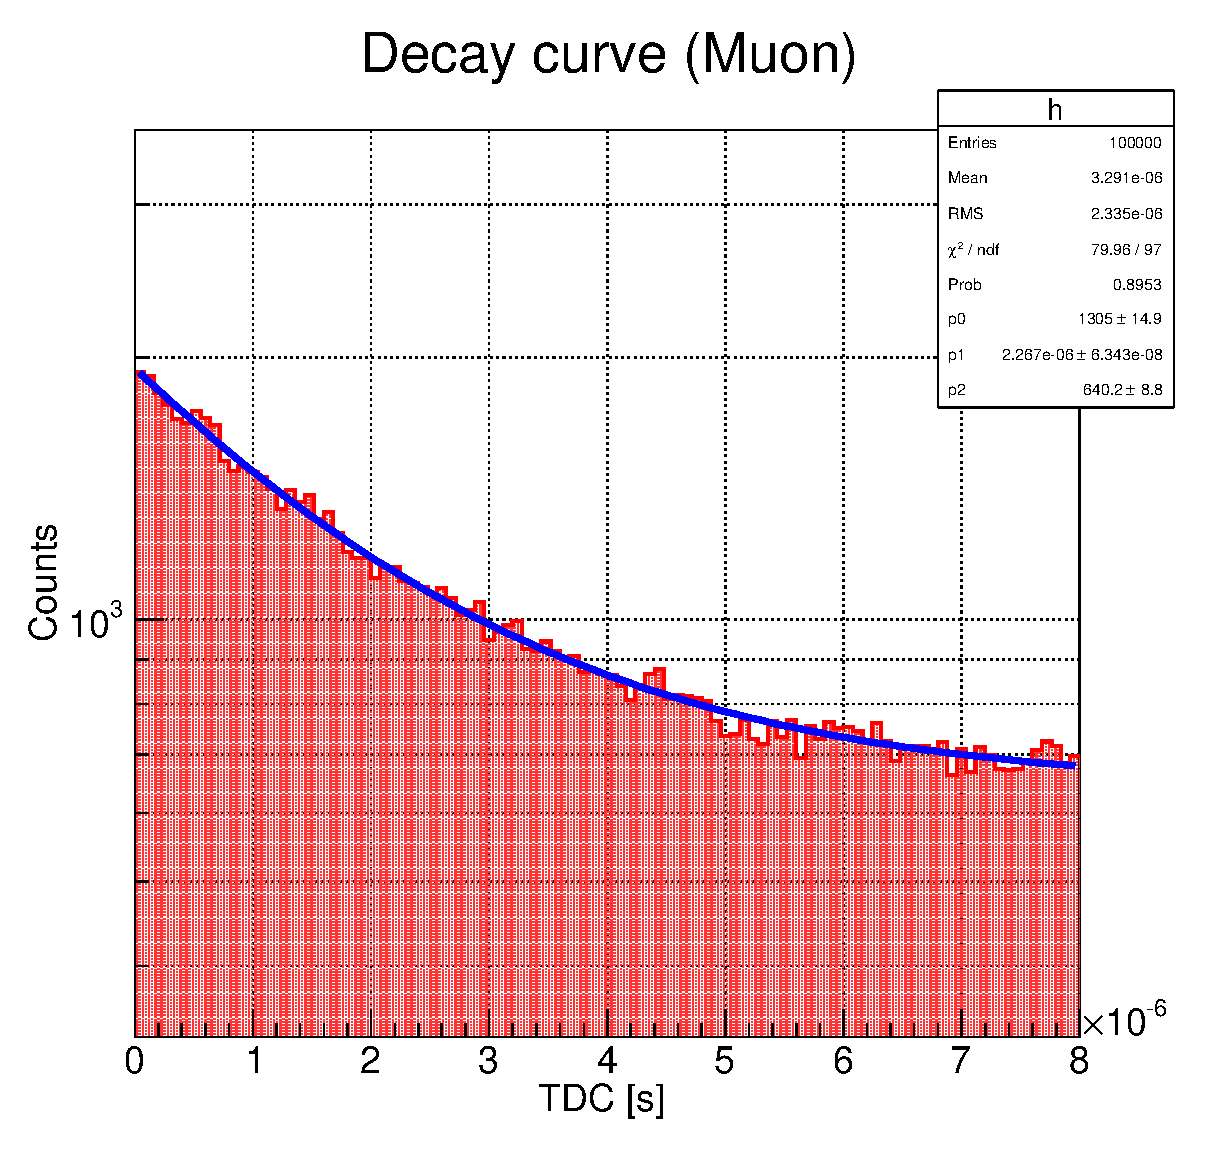
\includegraphics[width = 90mm]{./picture/ranfunsol2canvas1.eps}
	  \end{center}
	  \caption{\texttt{ranfunsol2.cpp}の実行結果}
	  \label{Fig:ranfunsol2canvas1}
	 \end{figure}

  \end{enumerate}
